% PhD thesis template, Lund University
% Originally designed for the Faculty of Science: Astronomy and Theoretical Physics
% Reformatted to work with Overleaf

% Layout and typesetting: Daniel Michalik, with Berry Holl, Helene Jönsson, Jonas Palm, Samuel Stenberg, Vidar Aspelin
% Implementation and documentation: Daniel Michalik, Samuel Stenberg
%
% Credits to the past generations of students who contributed to the original
% versions of this latex template, in particular Berry Holl.
% 
% Compilation instructions: use "xelatex" (necessary for support of the fonts
% used by Lund University. The fonts need to be installed first, see README.txt
% for instructions).
%
% If you use (pdf)latex instead, the default latex fonts will be used. 
% That would be a pity, cause the Garamond/Frutiger suggestion by the
% University looks much nicer for your thesis!
%
% Special command to automatically make Mac's TeXshop use xelatex for this file:
% !TEX TS-program = XeLaTeX
%
\documentclass[11pt]{book} 

% Hide all the usepackage commands and definitions in a preamble file.
% Normally you should not need to edit it.
% Non-breakable hyphen. Use for things like "(re-)print". 
\newcommand\nobrkhyph{\mbox{-}}

% Small caps serif font, for Paper numbers, ISBN, etc
\newcommand{\I}{\textrm{\scshape i}\xspace}
\newcommand{\II}{\textrm{\scshape ii}\xspace}
\newcommand{\III}{\textrm{\scshape iii}\xspace}
\newcommand{\IV}{\textrm{\scshape iv}\xspace}
\newcommand{\V}{\textrm{\scshape v}\xspace}
\newcommand{\VI}{\textrm{\scshape vi}\xspace}
\newcommand{\VII}{\textrm{\scshape vii}\xspace}
\newcommand{\VIII}{\textrm{\scshape viii}\xspace}
\newcommand{\IX}{\textrm{\scshape ix}\xspace}
\newcommand{\X}{\textrm{\scshape x}\xspace}
\newcommand{\ISBN}{\textrm{\scshape isbn}\xspace}
\newcommand{\ISSN}{\textrm{\scshape issn}\xspace}

% Must come in the beginning. Changes the spacing in the table of contents to look more pleasing
\usepackage{tocloft}
\setlength{\cftbeforepartskip}{5.0mm}
\setlength{\cftbeforechapskip}{2.0mm}
\setlength{\cftbeforesecskip}{0.0mm}

% Must come in the beginning. To calculate the total number of pages
\usepackage{pageslts}

%%%%%%%%%%%%%%%%%%%%%%%%%% Everything font-related %%%%%%%%%%%%%%%%%%%%%%%%%%%%%%%%%%%%%%%
\usepackage{ifxetex}

% Font selections - they are only used when you compile with xelatex (strongly recommended). If you use 
% pdflatex, the default latex fonts will be used, you will break the University graphical profile, and your
% thesis will look much much uglier.
%\usepackage[adobe-garamond]{mathdesign}
\ifxetex
	\usepackage{mathspec}
	\usepackage[no-math]{fontspec}
	\usepackage{xunicode}
	\usepackage{xltxtra}
    %\usepackage[adobe-garamond]{mathdesign}
    \usepackage[Adobe Garamond]{mathdesign}
	% Adobe Garamond Pro for serif fonts and maths, Frutiger as sans, according to LU graphical profile
	% Tables get monospaced numerals, text gets proportional numerals, mathmode gets uppercase monospaced numberals
	%\setmainfont[Mapping=tex-text,Numbers={OldStyle,Proportional}]{Adobe Garamond Pro}
	\setmainfont{AGaramondPro}[Path = ./fonts/AGaramondPro/, Mapping = tex-text, Numbers = {OldStyle, Proportional}, UprightFont = *-Regular.otf, BoldFont= *-Semibold.otf, ItalicFont=*-Italic.otf]
	\AtBeginEnvironment{tabular}{\addfontfeatures{Numbers={Monospaced}}}
	%\setsansfont{Frutiger LT Std 45 Light}
	%\setsansfont{FrutigerLTStd}[Path = ./fonts/Frutiger/, RomanFont=*-Roman.otf, BoldFont=*-Bold.otf, ItalicFont=*-Italic.otf, LightFont=*-Light.otf, LightItalicFont=*-LightItalic.otf]
	\setsansfont{FrutigerLTStd-Roman.ttf}[Path = ./fonts/Frutiger/, BoldFont=FrutigerLTStd-Bold.ttf, ItalicFont=FrutigerLTStd-Italic.ttf]
	
	%\setmathfont(Greek,Digits,Latin){Adobe Garamond Pro}
	%\setmathfont(Greek,Digits,Latin){AGaramondPro-Roman.otf}
	% mathspec is broken. The next eight lines work around that.
	\usepackage{etoolbox}
	\makeatletter
	\begingroup\lccode`~=`"
	\lowercase{\endgroup
	  \everymath{\let~\eu@active@quote}
	  \everydisplay{\let~\eu@active@quote}
	}
	\makeatother
\else
	% This is what is used for pdf latex. 
	% You can try \usepackage{ebgaramond} with (pdf)latex, however that does not have bold fonts ... !
	%\usepackage{ebgaramond}
	 \usepackage[utf8]{inputenc}
\fi
%%%%%%%%%%%% end font selections

% Support for greek (non-math non-italic) text, e.g. for units like mircometer: \textmu m 
\usepackage{textgreek}

% Additional font sizes \HUGE and \ssmall, needed for figure captions
\usepackage{moresize}

% figure captions in bold (i.e. "Figure 1" in bold), sans serif, smaller font size, hanging label, always starting on the left side
\usepackage{subfig}
\DeclareCaptionFont{ssmall}{\ssmall}
\DeclareCaptionFont{tiny}{\tiny}% "scriptsize" is defined by floatrow, "tiny" not
\captionsetup{margin=0em,font={ssmall,sf},labelfont={bf},format=hang,singlelinecheck=false} 

% figures centred, smaller font in tables, captions on top for tables
\usepackage{floatrow}
\DeclareFloatFont{tiny}{\tiny}% "scriptsize" is defined by floatrow, "tiny" not
\DeclareFloatFont{ssmall}{\ssmall}
\floatsetup[table]{font={footnotesize},position=top}
%%%%%%%%%%%%%%%%%%%%%%%%%%%%%%%%%%%% end fonts %%%%%%%%%%%%%%%%%%%%%%%%%%%%%%%%%%%%%%%%%%%%%%%%%%%%%%%

% For tables spanning the full text width
\usepackage{tabularx}

% For URLs use \url{<URL>}
\usepackage{url}

% Chapters should have numbers - a typical thesis consists of two chapters:
% One to introduce and summarize the research ("kappa"), and one for
% reproductions of the papers and manuscripts. No need to number them by default.
% If you need chapter numbers back, comment the following line.
%\renewcommand{\thesection}{\arabic{section}} 

% Sections and subsections have numbers, subsubsections etc do not.
\setcounter{secnumdepth}{3}

% Only chapters and sections appear in the table of contents, not subsections etc
\addtocontents{toc}{\protect\setcounter{tocdepth}{3}}

% Ensures that \cleardoublepage inserts empty pages without page number
\usepackage{emptypage} 

% For text macros (e.g., small caps macros)
\usepackage{xspace}

% For "Lorem Ipsum" style place holders
\usepackage{blindtext}

% For \includegraphics
\usepackage{graphicx}

% Nice looking tables with correct spacings 
\usepackage{booktabs}

% Tables spanning more than one page
\usepackage{longtable}
 
% Math symbols
\usepackage{amsfonts,mathrsfs,amsmath,amssymb}
\usepackage[ruled,vlined]{algorithm2e}
% To include the PDFs of the papers
\usepackage{pdfpages}

% For Natural Science students who use ADS. Save to have in any case.
\usepackage{auxiliary_textfiles/aas_macros}

% Hyphenation, support for different languages, last one is default
% Make sure to install the hyphenation packages for all languages you need
\usepackage[swedish,ngerman,english]{babel} 

% Reference in style of Natural Sciences
\usepackage[super, comma, sort]{natbib}

% Non-indented paragraphs with a small vertical space in-between
\parindent 0in
\parskip 3mm

% Paper size. Typically this works also fine when printed on A4 (text size is
% as print later, just the margins become wider to accommodate the too large
% sheets).
%% G5 format
%\usepackage[paperwidth=169mm,paperheight=239mm,total={13.3cm,19.6cm}, top=1.8cm, ignorehead, centering, footskip=\footskip+4mm ]{geometry}
\usepackage[paperwidth=169mm,paperheight=239mm,total={12.5cm,19.6cm}, top=1.8cm, ignorehead, centering, footskip=\footskip+4mm ]{geometry}
% If you prefer E5 (smaller) you can use this line instead. Also go to frontmatter.tex and change the datasheet from G5 to E5.
%% E5 format
%\usepackage[paperwidth=155mm,paperheight=220mm,total={12cm,18cm}, top=1.8cm, ignorehead, centering, footskip=\footskip+4mm ]{geometry}

% not every page needs to go to the same bottom line. Allows nicer page breaks.
\raggedbottom

% avoid orphan/widow lines. Lower this number if necessary to get a good layout.
\widowpenalty500
\clubpenalty500


% These command should allow figures to be placed close to where we define them, 
% thus we can influence the figure placement to some extent.
%% min page fraction that must be filled with text
%\renewcommand{\textfraction}{0.1} 
\renewcommand{\textfraction}{0.2}
%% max page fraction that a float may take at the top of the page
%\renewcommand{\topfraction}{0.9} 
\renewcommand{\topfraction}{1.0}
%% max page fraction that a float may take at the bottom of the page
%\renewcommand{\bottomfraction}{0.9}
\renewcommand{\bottomfraction}{1.0}
%% max page fraction that may be filled with floats
%\renewcommand{\floatpagefraction}{0.5}
\renewcommand{\floatpagefraction}{1.0}
%% maximum number of floats at the top of the page
\setcounter{topnumber}{1}
%% maximum number of floats at the bottom of the page
\setcounter{bottomnumber}{1}
%% maximum total number of floats on a page
\setcounter{totalnumber}{1}

% Figures can be kept in the same directory as the thesis, or in a Figure/
% directory, without need to specifying which of the two it is
\graphicspath{{figures/}}


%%%%%%%%%%%%%%%%%%%%%%%%%%%%%%%%%%%%%%%%%%%%%%%%%%%%%%%%%%%%%%%%%%%%
% define commands for chapters, sections, and subsections that do not 
% have a number, but are entered as candidates for the table of contents.
\newcommand\chap[1]{%
  \chapter*{#1}%
  \addcontentsline{toc}{chapter}{#1}
  \markboth{#1}{#1}
}
\newcommand\sect[1]{%
  \section*{#1}%
  \addcontentsline{toc}{section}{#1}
  \markright{#1}
}
\newcommand\subsect[1]{%
  \subsection*{#1}%
  \addcontentsline{toc}{subsection}{#1}
}
\newcommand\subsubsect[1]{%
  \subsubsection*{#1}%
  \addcontentsline{toc}{subsubsection}{#1}
}


%%%%%%%%%%%%%%%%%%%%%%%%%%%%%%%%%%%%%%%%%%%%%%%%%%%%%%%%%%%%%%%%%%%%
% Define nice headers and footers
% To keep the thesis non-cluttered we only put the page number into the footer,
% and avoid headers
\usepackage{fancyhdr}
\fancyheadoffset{0cm}
\pagestyle{plain}
%page number in the foot centre 
\cfoot{\fancyplain{\thepage}{}}

% You want to use headers? Here is some things for your inspiration:
%\renewcommand{\chaptermark}[1]%
%               {\markboth{#1}{#1}}
%\renewcommand{\sectionmark}[1]%
%               {\markright{\thesection\ #1}}
%\renewcommand{\chaptermark}[1]{\markboth{\thechapter\ #1}{\thechapter\ #1}}
%\lhead[\fancyplain{}{\thepage}]%
%      {\fancyplain{}{\textsl\rightmark}}
%\rhead[\fancyplain{}{\textsl\leftmark}]%
%      {\fancyplain{}{\thepage}}
% Contents and references should not print a uppercase header on their second pages
%\usepackage{etoolbox}
%\patchcmd{\tableofcontents}{\MakeUppercase\contentsname}{\contentsname}{}{}
%\patchcmd{\tableofcontents}{\MakeUppercase\contentsname}{\contentsname}{}{}
%\patchcmd{\bibsection}{\MakeUppercase{\bibname}}{\bibname}{}{}
%\patchcmd{\bibsection}{\MakeUppercase{\bibname}}{\bibname}{}{}

% References should be a section of the summary text, with number and all ...
\renewcommand\bibsection{\chap{\bibname}\markright{\bibname}}

% If you want to use a box to summarize your papers, try \begin{thesisbox}{title}
\usepackage{tcolorbox}
\tcbuselibrary{skins}
\newtcolorbox{thesisbox}[2][]{
oversize=-2.5cm,
  enhanced,
  attach boxed title to top left={yshift=-2ex,xshift=6ex},
  before skip=1em,
  after skip=1em,
  colframe=black,
  colback=white,
  fonttitle=\bfseries, 
  colbacktitle=white,
  coltitle=black,
  boxed title style={
    boxrule=0pt,
    colframe=white,
    },
  title=#2,
  #1}
\newcounter{exa}

% ********************************************************************
% Re-usable information (title page, datasheet), please edit the file parameters.tex to include correct information
\newcommand{\myName}{Ganepola Arachchige Thushadh Wijesekere}
\newcommand{\myYear}{2028}
\newcommand{\myMainTitle}{Safety Distances from Hydrogen Jet Flames}
\newcommand{\mySubTitle}{}

% Compact combination of combining title and subtitle, used in datasheet and as
% chapter title for the main part.
\newcommand{\myTitle}{\myMainTitle\ \mySubTitle} 

\newcommand{\myFaculty}{Faculty of Engineering}
\newcommand{\myDepartment}{Division of Fire Safety Engineering}
\newcommand{\myAddress}{Jon Ericssons Vag 1\\SE--221 00 LUND\\Sweden} % Three lines maximum!

% Only change once you are ready. Looks to scary otherwise.
% This might be the degree you are obtaining: Thesis for the degree of Doctor of Philosophy
\newcommand{\myDegree}{Doctoral Dissertation}
\newcommand{\myAdvisors}{Prof. Patrick van Hees, Dr. Marcus Runefors}
\newcommand{\myOpponent}{Prof. Gammal och Grå}

\newcommand{\myDefenceAnnouncement}{%
	To be presented, with the permission of the
	\myFaculty\xspace of Lund University, for public criticism at LINXS (Delta 5, floor 5, IDEON building)
	on friday, the 30th of October \myYear\xspace at 10:15. }
\newcommand{\myCoverFront}{%
	{\bf Cover illustration front:} 
	Cool figure by bla and bla.}
\newcommand{\myCoverBack}{%
	{\bf Cover illustration back:} Another cool image by bla.}
\newcommand{\myFundingInformation}{%
	{\bf Funding information:} 
	The thesis work was financially supported by the Swedish Research Council.}
	
\newcommand{\quotes}[2]{\begin{flushright}\textit{#1}\\--- #2\end{flushright}}
% Series number. Astronomy users:
% Series: {\scshape lunfd6/(nfas}-1048)/1-\myPages/(\myYear)}
% where you increment the number 1048 by one wrt to last thesis at the department
% 
% Your department maybe uses something else, probably an ISSN number? 
%\newcommand{\mySeries}{%
%	\ISSN: $<$ISSN number$>$}

\newcommand{\myISBNprint}{123456789}
\newcommand{\myISBNpdf}{123456789}
\newcommand{\myFormSignDate}{2020-09-18}

% total page number is computed automatically:
\newcommand{\myPages}{\lastpageref{LastPages}}

\newcommand{\myFormDefenceDate}{2020-10-30}
\newcommand{\myFormKeywords}{%
	statistical thermodynamics, molecular simulation, Markov chains, Monte Carlo simulations, electrostatics, Ewald summation, ionic liquids, electric double layer supercapacitors}

% Write a short english abstract of the thesis here, goes into the data sheet page 4. 
\newcommand{\myAbstract}{
\blindtext
}%

% --- Shortcut thesis commands for paper references and titles ---
% Included papers - only need to type this once
\newcommand{\PaperIauthor}{\textbf{S. Doctor}, B. Someone}
\newcommand{\PaperIIauthor}{\textbf{S. Doctor}, B. Someone, C Another}

\newcommand{\PaperIref}{\textit{The Journal of Physical Chemistry A}, 2020, 124(19), pp. 3943-3946}
\newcommand{\PaperIIref}{\textit{Physical Chemistry Chemical Physics}, 2020, 22(24), pp. 13659-13665}

\newcommand{\PaperItitle}{Title paper 1}
\newcommand{\PaperIItitle}{Title paper 2}

% Declare other commands such as useful math operators:
\DeclareMathOperator{\erfc}{erfc}
\DeclareMathOperator{\erf}{erf}

% Not included papers, in case you want to list them
%\newcommand{\PaperNotIncIauthor}{C. Coauthor, \textbf{X. Someone}}
%\newcommand{\PaperNotIncIref}{Journal for \ldots}
%\newcommand{\PaperNotIncItitle}{Boring matter}
% --- END reusable thesis commands ---

\begin{document}

%%%%%%%%%%%%% First pages with thesis title etc %%%%%%%%%%%%%%%%%%%%%%%%%%%%%%%%
% First six pages are contained in a separate file. Normally you should not
% need to edit it.
% This file contains the layout of the first six pages and the explanation text
% of a compilation thesis. 

%%%%%%%%%%%%% FIRST PAGES WITH THESIS TITLE ETC %%%%%%%%%%%%%%%%%%%%%%%%%%%%%%%%
\frontmatter % roman numbers

% Page one: Title only
\thispagestyle{empty} % no page number
\begin{center}
\vspace*{5cm}
{\Large \myMainTitle}
%\\
%{\large \mySubTitle}
\end{center}

% Page two: empty. Empty space is important

%%%%%%%%%%%%%%%%%%%%%%%%%%%%%%%%%%%%%%%%%%%%%%%%%%%%%%%%%%%%%%%%%%%%%%%
% Page three: title page with small text (spikningsblad)

\cleardoublepage
\thispagestyle{empty} % no page number
~
\vfill
\begin{center}
{\HUGE \myMainTitle}
\\[2mm]
{\huge \mySubTitle}

\vfill
{\myName}

\vfill
% black and white (default):

\includegraphics[width=0.25\textwidth]{LundUniversity_C2line_BLACK.eps}

% Colour text in white so that the spacing is the same as on page three, but with less clutter

\vspace{10mm}
{\large \myDegree}\\
{\large Thesis advisors: \myAdvisors}\\
{\large Faculty opponent: \myOpponent}\\
\vfill
{\footnotesize
\myDefenceAnnouncement
}
\\
\end{center}
\vfill

%%%%%%%%%%%%%%%%%%%%%%%%%%%%%%%%%%%%%%%%%%%%%%%%%%%%%%%%%%%%%%%%%%%%%%%
% Page four: data sheet
\newpage \thispagestyle{empty} % no page number
%Either include datasheet texfile (will be filled in automatically), or a pdf
%containing datasheet (text needs to be already in it, edit
%sheetPDF_editable.pdf). Use one of the next two lines: 
\newcounter{aformdx}
\newcounter{aformdy}
\newcounter{aformx}
\newcounter{aformy}
\newcounter{aformtx}
\newcounter{aformtdx}
\newcounter{aformty}
\def\aformw{358}
\def\aformwhalf{\aformw / 2}
\def\aformwquart{\aformw / 4}
\def\aformwthreeq{\aformw / 4 * 3}
\def\aformh{517}
\def\aformb{23}
\def\aformlinew{0.4pt}
\def\aformrowh{20}
\def\aformRowh{24}
\newcommand\aformhline
{\put(\value{aformx},\value{aformy}){\line(1,0){\value{aformdx}}}}
\newcommand\aformvline
{\put(\value{aformx},\value{aformy}){\line(0,-1){\value{aformdy}}}}
\newcommand\aformvlinec
{\put(\value{aformx},\value{aformy}){\line(0,-1){16.25}}}
\newcommand\aformboxbase[5]
{
  \setcounter{aformtx}{\value{aformx}}
  \setcounter{aformtdx}{\value{aformdx}}
  \setcounter{aformty}{\value{aformy}}
  \addtocounter{aformtx}{#1}
  \addtocounter{aformtdx}{-#2}
  \addtocounter{aformty}{-#3}
  \put(\value{aformtx},\value{aformty})
  {
    \parbox[t]{\value{aformtdx}pt}
    {{\sf\tiny #4}{\scriptsize #5\par}}
  }
}
\newcommand\aformbox[2]{\aformboxbase{2}{11}{8}{#1}{#2}}
\newcommand\aformBox[2]{\aformboxbase{2}{11}{8}{#1}{#2}}

\begin{center}
\begin{picture}(\aformw,542)(0,0)
\linethickness{\aformlinew}
\put(0,\aformb){\framebox(\aformw,\aformh){}}
\put(-14,200){\rotatebox{90}{\parbox{200pt}
{\sf\tiny
DOKUMENTDATABLAD
enl SIS 61 41 21\\
}}}
\setcounter{aformx}{0}
\setcounter{aformy}{\aformb}
\addtocounter{aformy}{\aformh}
\setcounter{aformdx}{\aformwhalf}
\aformbox{Organization}
{\\
{\bf LUND UNIVERSITY}\vspace{0.1cm}
\\
{\myDepartment\\
\myAddress}
}
\setcounter{aformdy}{\aformrowh}
\addtocounter{aformdy}{\aformrowh}
\addtocounter{aformdy}{\aformrowh}
\addtocounter{aformdy}{\aformRowh}
\setcounter{aformx}{\aformwhalf}
\aformvline
\setcounter{aformx}{0}
\addtocounter{aformy}{-\aformrowh}
\addtocounter{aformy}{-\aformrowh}
\addtocounter{aformy}{-\aformRowh}
\aformbox{Author(s)}{\\\myName}
\setcounter{aformdy}{\aformrowh}
\aformhline
\addtocounter{aformy}{\aformrowh}
\addtocounter{aformy}{\aformrowh}
\addtocounter{aformy}{\aformRowh}
\setcounter{aformx}{\aformwhalf}
\aformbox{Document name}{\\{\bf LICENTIATE THESIS}}
\addtocounter{aformy}{-\aformrowh}
\aformhline
\aformbox{Date of disputation}{\\\myFormDefenceDate}
\setcounter{aformx}{\aformwhalf}
\aformhline
\addtocounter{aformy}{-\aformrowh}
\addtocounter{aformdy}{\aformRowh}
\aformbox{Sponsoring organization}{}
\aformhline
\addtocounter{aformy}{-\aformRowh}
\addtocounter{aformy}{-\aformrowh}
\setcounter{aformx}{0}
\setcounter{aformdx}{\aformw}
\aformhline
\aformbox{Title and subtitle }{\\\myTitle}
\addtocounter{aformy}{-\aformRowh}
\setcounter{aformx}{0}
\aformhline
\aformBox{Abstract}
{\\
{\parskip0pt\parindent1em
\myAbstract
}
}
\setcounter{aformy}{\aformb}
% Correspond to one minus each in the bottom section
\addtocounter{aformy}{\aformRowh}
\addtocounter{aformy}{\aformRowh}
\addtocounter{aformy}{\aformRowh}
\addtocounter{aformy}{\aformRowh}
\addtocounter{aformy}{\aformrowh}
\addtocounter{aformy}{\aformrowh}
\addtocounter{aformy}{10}
\addtocounter{aformy}{10}
\aformhline
\aformbox{Key words}
{
\\\myFormKeywords
}
\addtocounter{aformy}{-\aformRowh}
\addtocounter{aformy}{-10}
\aformhline
\aformbox{Classification system and/or index terms (if any)}{}
\addtocounter{aformy}{-\aformRowh}
\aformhline
\aformbox{Supplementary bibliographical information}{}
\setcounter{aformx}{\aformwthreeq}
\setcounter{aformdx}{\aformwquart}
\setcounter{aformdy}{\aformRowh}
\aformvline
\aformbox{Language}{\\English}
\addtocounter{aformy}{-\aformRowh}
\setcounter{aformx}{0}
\setcounter{aformdx}{\aformw}
\aformhline
\aformbox{ISSN and key title}{}
\setcounter{aformx}{\aformwthreeq}
\addtocounter{aformdy}{10}
\aformvline
\addtocounter{aformdy}{-10}
\aformbox{ISBN}{\\\myISBNprint\xspace(print)\\\myISBNpdf\xspace(pdf)}
\addtocounter{aformy}{-\aformRowh}
\addtocounter{aformy}{-10}
\setcounter{aformx}{0}
\aformhline
\aformbox{Recipient's notes}{}
\setcounter{aformx}{\aformwhalf}
\setcounter{aformdy}{\aformrowh}
\addtocounter{aformdy}{\aformrowh}
\aformvline
\aformbox{Number of pages}{\\\myPages}
\setcounter{aformx}{\aformwthreeq}
\aformbox{Price}{}
\setcounter{aformdy}{\aformrowh}
\aformvline
\addtocounter{aformy}{-\aformrowh}
\setcounter{aformx}{\aformwhalf}
\setcounter{aformdx}{\aformwhalf}
\aformhline
\aformbox{Security classification}{}
\setcounter{aformx}{0}
\setcounter{aformdx}{\aformw}
\addtocounter{aformy}{-\aformrowh}
\addtocounter{aformy}{-4}
\aformbox{}
{\scriptsize I, the undersigned, being the copyright owner of the abstract of the
above-mentioned dissertation, hereby grant to all reference sources
the permission to publish and disseminate the abstract of the
above-mentioned dissertation.
}
\addtocounter{aformy}{-\aformRowh}
\addtocounter{aformy}{-20}
\aformbox{
\hspace{0pt}
%\put(44,1){\includegraphics{images/signature}} %Media-Tryck does not want this to be included as a graphic
}{}
\aformbox{\rm
\scriptsize
Signature \underline{\hskip 140pt}\hfill Date \underline{\hskip 80pt}
}{}
\addtocounter{aformy}{1}
\aformbox{}{\hskip 280pt \scriptsize \myFormSignDate}
\end{picture}
\end{center}

%\addtocounter{pages}{1} 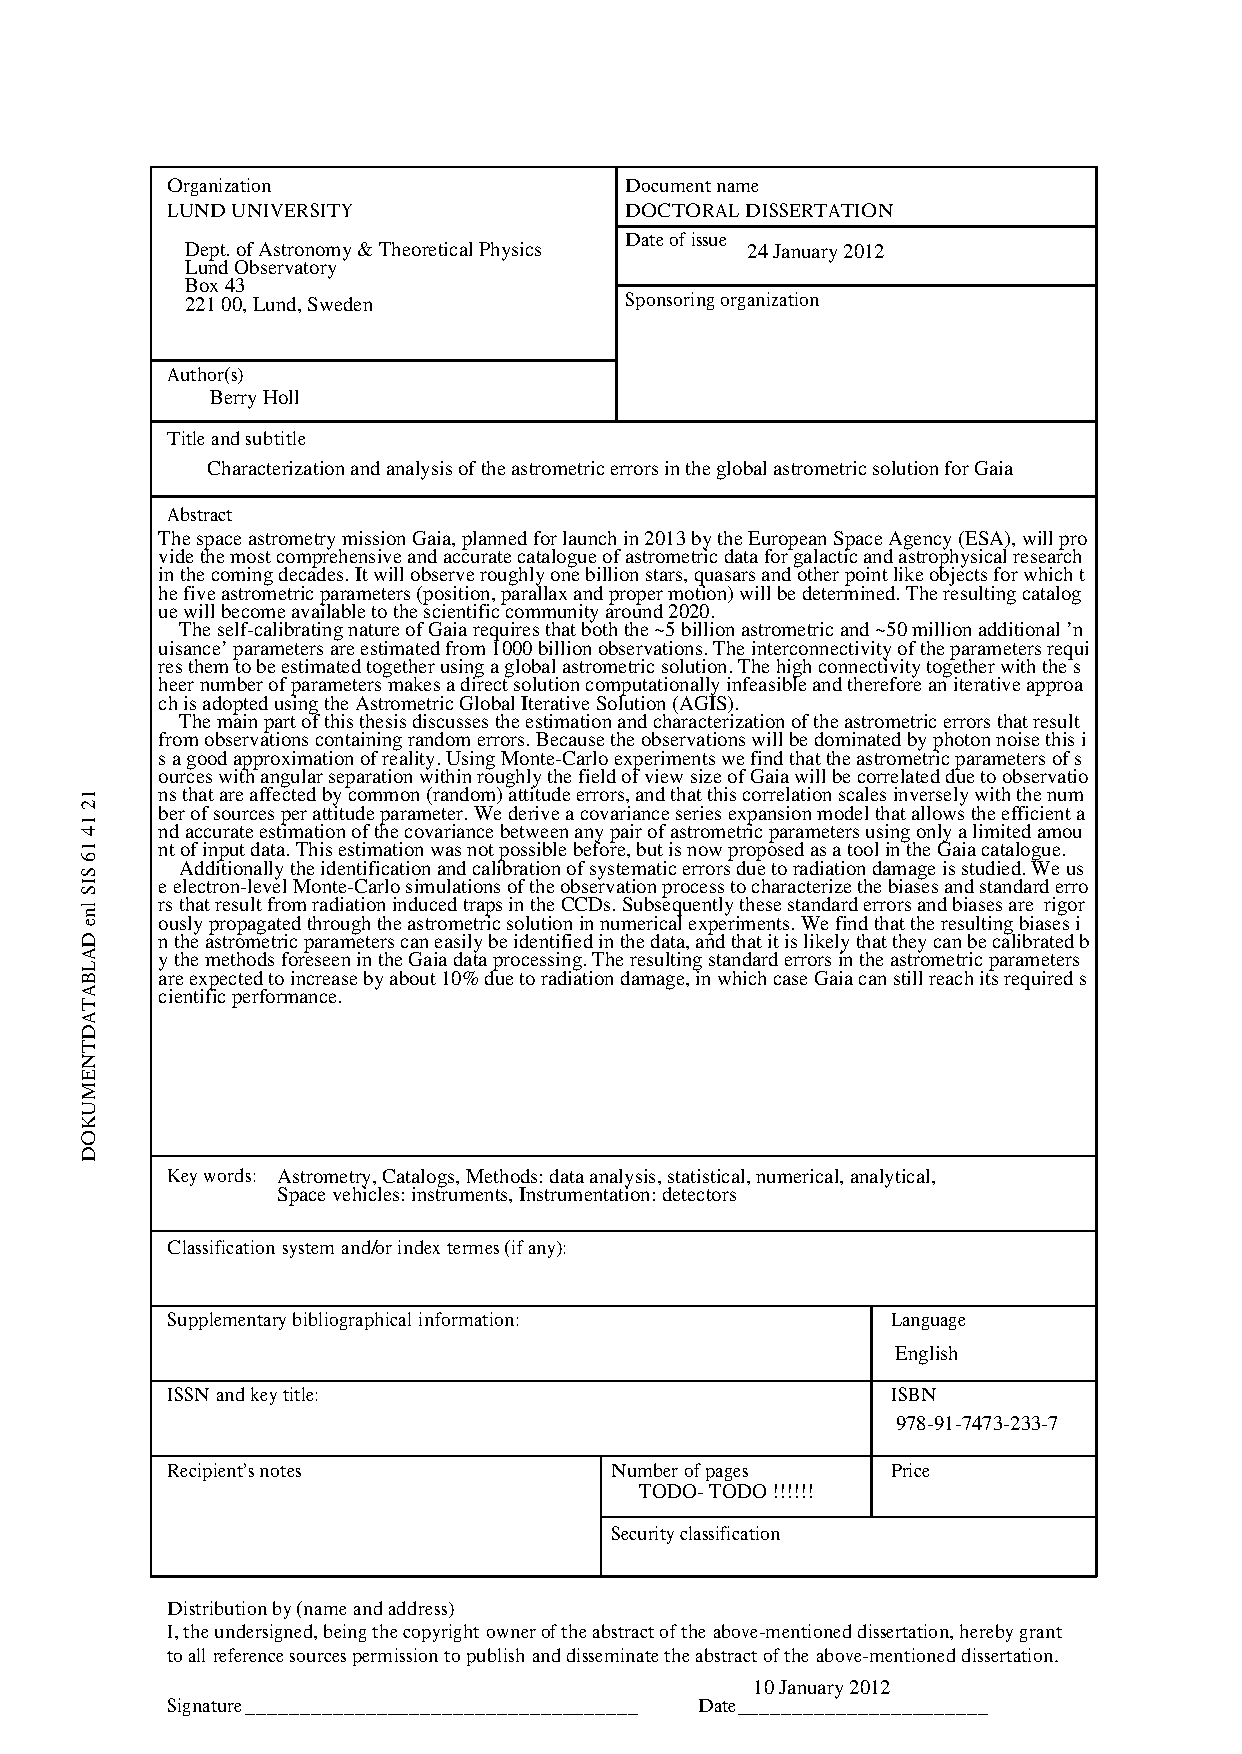
\includepdf[pages=1-1]{datasheetPDF_editable}

%%%%%%%%%%%%%%%%%%%%%%%%%%%%%%%%%%%%%%%%%%%%%%%%%%%%%%%%%%%%%%%%%%%%%%%
% Page five: title and author, without small text. Looks good!

\cleardoublepage
\thispagestyle{empty} % no page number
~
\vfill
\begin{center}
{\HUGE \myMainTitle}
\\[2mm]
{\huge \mySubTitle}

\vfill
{by \myName}

\vfill
% black and white (default):

\includegraphics[width=0.25\textwidth]{LundUniversity_C2line_BLACK.eps}

% Colour text in white so that the spacing is the same as on page three, but with less clutter
\color{white}{
\vspace{10mm}
{\large \myDegree}\\
{\large Thesis advisors: \myAdvisors}\\
{\large Faculty opponent: \myOpponent}\\
\vspace{1cm}
{\footnotesize
\myDefenceAnnouncement
}
}
\\
\end{center}
\vfill


%%%%%%%%%%%%%%%%%%%%%%%%%%%%%%%%%%%%%%%%%%%%%%%%%%%%%%%%%%%%%%%%%%%%%%%
% Page six: Cover image description, ISBN, copyright
\newpage 
\thispagestyle{empty} % no page number
%~
%\vfill
\vspace{-15mm}
A licentiate thesis at a university in Sweden takes either the form of a single,
cohesive research study (monograph) or a summary of research papers
(compilation thesis), which the licentiate student has written alone or together
with one or several other author(s). 

In the latter case the thesis consists of two parts. An introductory text puts
the research work into context and summarizes the main points of the papers.
Then, the research publications themselves are reproduced, together
with a description of the individual contributions of the authors. The
research papers may either have been already published or are manuscripts at
various stages (in press, submitted, or in draft). 

\vfill
{\small
\myCoverFront\\
\\
\myCoverBack\\
\\
\myFundingInformation


\vspace{5mm}
\copyright\, \myName~\myYear\\
\\
\myFaculty, {\myDepartment}
\\
\\
\ISBN: \myISBNprint~(print)\\ % ISBN av svenska ISBN centralen
\ISBN: \myISBNpdf~(pdf)\\ % ISBN av svenska ISBN centralen
%\mySeries\\
\\
Printed in Sweden by Media-Tryck, Lund~University, Lund~\myYear


\includegraphics[width=0.5\textwidth]{miljologotyper}
}


% ===============================================================
% ===================== INSPIRATIONAL QUOTE:  ===================
% ===============================================================
\newpage
\thispagestyle{empty} % No page number on quote page
~
\vspace{140pt}
\begin{flushright}
\textit{Dedicated to\\Humpty -- Dumpty\\bla bla blat}
\end{flushright}


\cleardoublepage


%%%%%%%%%%%%%%%%%%%%%%%%%%%%%%  Table of contents   %%%%%%%%%%%%%%%%%%%%%%%%%%%%%%%%%%%%%%%
\setcounter{page}{1} % Page Roman 1 of the frontmatter
\setcounter{tocdepth}{1}
\tableofcontents
% no page number on toc page:
\addtocontents{toc}{\protect\thispagestyle{empty}}


%%%%%%%%%%%%%%%%%%%%%%%%%%%%%%%%% List of publications %%%%%%%%%%%%%%%%%%%%%%%%%%%%%%%%%%%%%%
% Have a long list and want to start on the left page? Here, have a special
% chapter heading for that!
%\addcontentsline{toc}{part}{Part 1: Summary}
%\renewcommand{\chapterheadstartvskip}{}
%{\let\cleardoublepage\relax \let\chapterheadstartvskip\nop 

\newpage
\sect{List of publications\label{sec:paperlist}}
This thesis is based on the following publications, referred to by their Roman numerals:
\vspace{2mm}

{
% Normal font size in this table, afterwards continue with slightly smaller table font size stated in preamble
\floatsetup[table]{font={normalsize},position=top}
\begin{tabularx}{\textwidth}{rX}
% Normal font size in this table, afterwards continue with slightly smaller table font size stated in preamble
\normalsize
\I	  & {\bf \PaperItitle}\\[2mm]
	  & \PaperIauthor\\
          & \PaperIref\\[6mm] 

\II	  & {\bf \PaperIItitle}\\[2mm]
	  & \PaperIIauthor\\
          & \PaperIIref\\[6mm]
\end{tabularx}

All papers are reproduced with permission of their respective publishers.
%Or maybe you need to be more specific? Like: Paper~I and II reproduced with permission \copyright\ ESO\\

% Publications not included in this thesis:
% \vspace{2mm}
%
% \begin{tabularx}{\textwidth}{rX}
% {\sc \phantom{vi}}   & {\bf \PaperNotIncItitle}\\[2mm]
%	  & \PaperNotIncIauthor\\
%          & \PaperNotIncIref\\[5mm] 
%
%\end{tabularx}
%
} % End large font tables, continue with font size stated in preamble


                 
% ===============================================================
% ====================== Acknowledgements:  =====================
\newpage
\sect{Acknowledgements}
\blindtext

% ===============================================================
% ===================== POPULAR SUMMARIES:  =====================

%----------------- SUMMARY IN SWEDISH --------------------
\newpage
\selectlanguage{swedish}
\sect{Populärvetenskaplig sammanfattning på svenska}
\blindtext

% ===============================================================
% ======================= SUMMARY CHAPTER   =====================
% Back to British spelling
\selectlanguage{english}
% Need to add hyphenation corrections? Do like this:
% \hyphenation{as-tro-me-try ana-lysis}

% Page numbers arabic 
\mainmatter
% Reset table counters to not count the publications table
\setcounter{table}{0} 
% Rest page counters, this is where it all starts!
\setcounter{page}{1}

\chap{\myTitle}
% Fancy a quote?
\newpage

%%%%%%%%%%%%%%%%%%%%%%%%%%%%%%%%%%%%%%%%% Actual kappa %%%%%%%%%%%%%%%%%%%%%%%%%%%%%%%%%%%%%%%%%
\chapter{Introduction}
This is the first line I have written on my phd thesis.\footnote{Unfortunately, this line will be deleted}

I also added this line from vim-tex. Vim-tex is awesome \\

seriously, it is so awesom \\

seriously, it is so awesome.
\vfill

\newpage
\begin{figure}
    \centering
    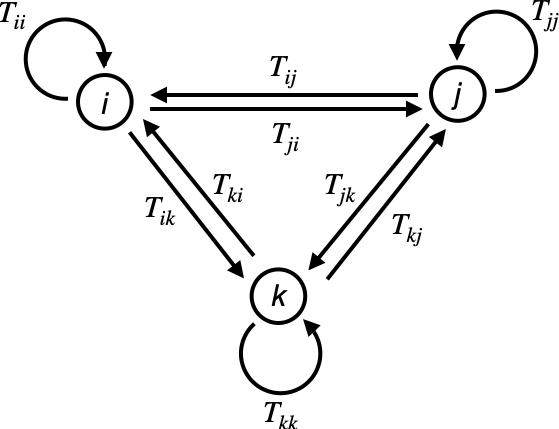
\includegraphics[scale=0.5]{figures/graph.png}
    \caption{Caption}
    \label{fig:my_label}
\end{figure}

\chapter{Cool Stuff}
\begin{tcolorbox}[colback=yellow!10!white,colframe=red!50!black,fonttitle=\scshape,
  titlerule=0pt,
  title={\refstepcounter{exa}example~\theexa: Title of Example},
  title style={fill=yellow!10!white},
  coltitle=white, %red!50!black
  drop shadow]
  Hi, i am a yellow example
  \begin{center}
    \centering
    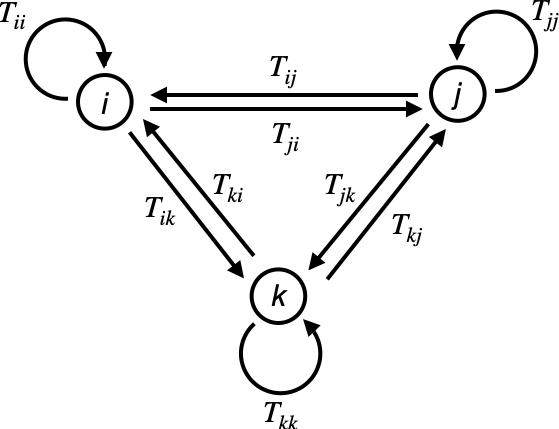
\includegraphics[width=0.99\textwidth]{figures/graph.png}
    \label{example:dice_entropy}
  \end{center}
\end{tcolorbox}
In example \ref{example:dice_entropy}

\begin{thesisbox}{The important concept}
\blindtext
\end{thesisbox}
\blindtext
\chapter{Research and Outlook}
\blindtext
%%%%%%%%%%%%%%%%%%%%%%%%%%%%%%%%%%%%%%%%%%%%%%%%%%%%%%%%%%%%%%%%%%%%%%%%%%%%%%%%%%%%%%%%%%%%%%%%
% ===============================================================
% ====================== References:  ===========================

% Bibliography renamed to references
\renewcommand{\bibname}{References}
\bibliographystyle{unsrtnat}
\bibliography{refs}  % Link to bibtex file
% ===============================================================
% ====================== Part II: Scientific publications  ======
% ===============================================================

\chap{Scientific publications}
\sect{Author contributions}

%Co-authors are abbreviated as follows: \\
%Foo Bar (FB), \ldots.

\subsect{Paper~\I: \PaperItitle}

I participated in developing the theory and wrote the simulation software. I participated in writing the manuscript.

\subsect{Paper~\II: \PaperIItitle}

I participated in developing the theory and writing simulation software. I participated in writing the manuscript.

%%%%%%%%%%%%%%%%%%%%%%%%%%%%%%%%%%%%%%%%%%%%%%%%%%%%%%%%%%%%%%%%%%%%
% Include the papers. Try this out once in the beginning, but maybe disable it
% for the main phase of your writing - it takes too long to compile otherwise.

% Papers should be formatted to G5 and then included! (Paula can do this for you)


%%%%%%%%%%%%%%%%%%%%%%%%%%%%%%%%%%     First paper    %%%%%%%%%%%%%%%%%%%%%%%%%%%%%%%%%%%%%%%
\cleardoublepage
\addcontentsline{toc}{section}{Paper~\I: {\PaperItitle}} % <<<<<<<<<<<<<<<<< Change the two Roman numbers here
\thispagestyle{empty}
\vspace*{20mm} %increase by 2cm each time. % <<<<<<<<<<<<<<<<<<<<<<<<<<<<<<<< Important
\begin{minipage}{8cm}

\end{minipage}%
\hfill{ 
\fontsize{20}{30}\selectfont {\bf Paper~\I}}\marginpar{\rule[-4mm]{50mm}{14mm}} % Change the Roman number here
\vfill
\textbf{S. Doctor} and B. someone\\
An Exact Ewald Summation Method in Theory and Practice\\
\textit{The Journal of Physical Chemistry A}, 2020, 124(19), pp. 3943-3946\\
Reproduced with permission from \textit{J. Phys. Chem. A}\\
Copyright 2020 American Chemical Society.

%Second: The PDF itself
\cleardoublepage
% Include the PDF. Comment this while writing the thesis, only add later. 
% Options are: all pages, scaled to full width (use 0.95 if that is too high for some reason), with thesis page number

\includepdf[pages=-,pagecommand={}]{papers/paperI.pdf}
% One additional option could be useful: To cut away the margins of the included PDFs use:
% clip,viewport=<left> <bottom> <right> <top>
% To determine the four numbers you can use the ./determineViewport.sh script in the thesis directory. 



%%%%%%%%%%%%%%%%%%%%%%%%%%%%%%%%%%     Second paper    %%%%%%%%%%%%%%%%%%%%%%%%%%%%%%%%%%%%%%%

\cleardoublepage
\addcontentsline{toc}{section}{Paper~\II: {\PaperIItitle}} % <<<<<<<<<<<<<<<<< Change the two Roman numbers here
\thispagestyle{empty}
\vspace*{34mm} %increase by 14mm each time. % <<<<<<<<<<<<<<<<<<<<<<<<<<<<<<<< Important
\begin{minipage}{8cm}
% Optional text, 1 line max, can also be left empty
%Conference poster in Appendix A.1
\end{minipage}%
\hfill{ 
\fontsize{20}{30}\selectfont {\bf Paper~\II}}\marginpar{\rule[-4mm]{50mm}{14mm}} % Change the Roman number here
\vfill
\textbf{S. Doctor}, B. someone, C. another and D. another\\
Grand canonical simulations of ions between charged conducting surfaces using exact 3D Ewald summations\\
\textit{Physical Chemistry Chemical Physics}, 2020, 22(24), pp. 13659-13665\\
Reproduced from \textit{Phys. Chem. Chem. Phys.} with permission from the PCCP Owner Societies.

\cleardoublepage

\includepdf[pages=-,pagecommand={}]{papers/paperII.pdf}



%%%%%%%%%%%%%%%%%%%%%%%%%%%%%%%%%% Repeat for all papers ..   %%%%%%%%%%%%%%%%%%%%%%%%%%%%%%%%%%%%%%%%%%%%


%%%%%%%%%%%%%%%%%%%%%%%%%%%%%%%%%%%%%%%%%%%%%%%%%%%%%%%%%%%%%%%%%%%%%%%%%%%%%%%%%%%
% Finally, an optional appendix, for example if your posters are helpful in any way.
%\cleardoublepage
%\appendix
%\thispagestyle{empty}
%\vspace*{4cm} %increase by 2cm each time. %<<<<<<<<<<<<<<<<<<<<<<<<<<<<< Important
%\hfill{ %\fontspec{Frutiger}
%\fontsize{20}{30}\selectfont {\bf Appendix}}\marginpar{\rule[-4mm]{50mm}{14mm}}
%\vfill

%\appendix
%\chap{Appendix: Conference posters}
%\section*{Poster 1:}
%Media-Tryck's suggestion to a poster layout, can be downloaded from \url{https://bildweb.srv.lu.se/login/}.
%Presented 2067 at the \emph{Symposium for time travel} 
%in Berlin, Germany. For further details refer to Paper~\I and
%Sect.~\ref{sec:mainresults}.

% include poster itself. Cropping works as described above for the papers.
%\includepdf[pages=-,width=\paperwidth-10mm]{posterMediaTryck.pdf} %smaller margin, works fine when printing (hopefully ;) Hallå, Jonas!)

\end{document}
